\appendix
\bibliographystyle{IEEEtran}
\bibliography{svp}
\chapter{Model predictions}
\label{appendix:model_predictions}
The following figures are X-ray images from the test part of dataset. Ground truth labels are marked by pink color and the model predictions are in green. Each bounding box prediction has corresponging confidence attached to it.
\begin{figure}
    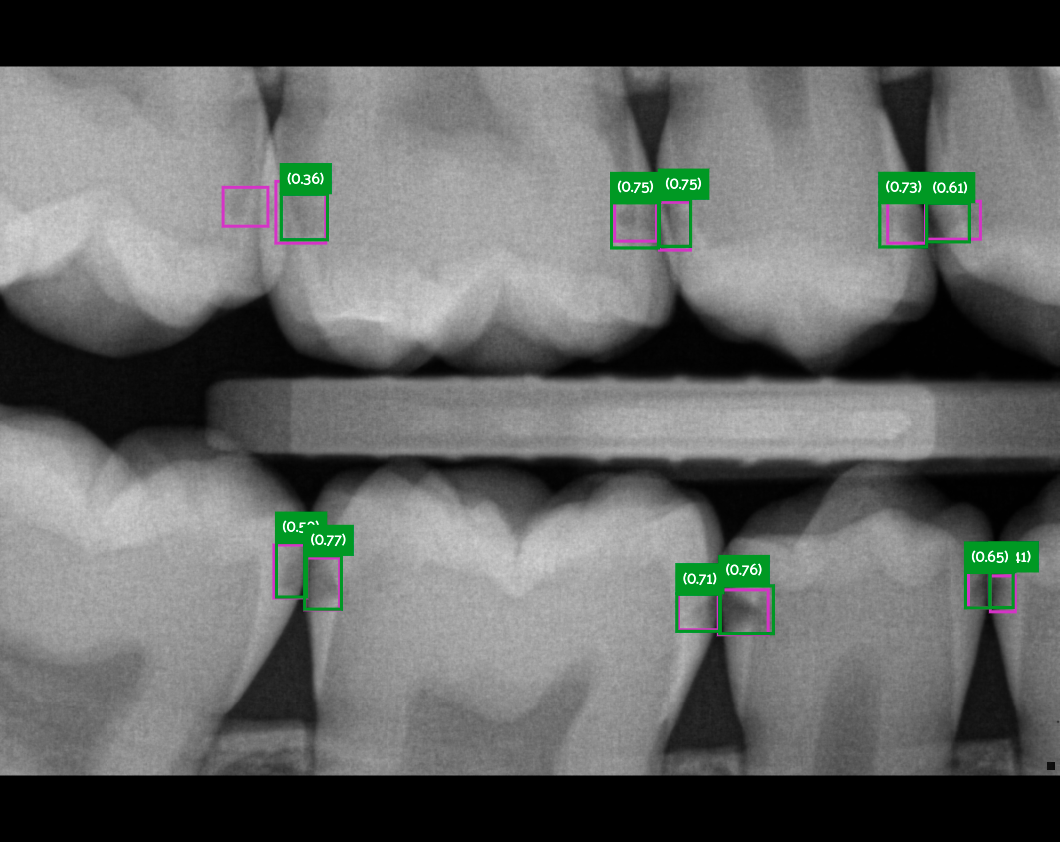
\includegraphics[width=0.9\linewidth]{images/no_rest1.png}
    \caption{X-ray image with ground truth boxes and model's predictions}
    \label{fig:pred_img1}
\end{figure}

\begin{figure}
    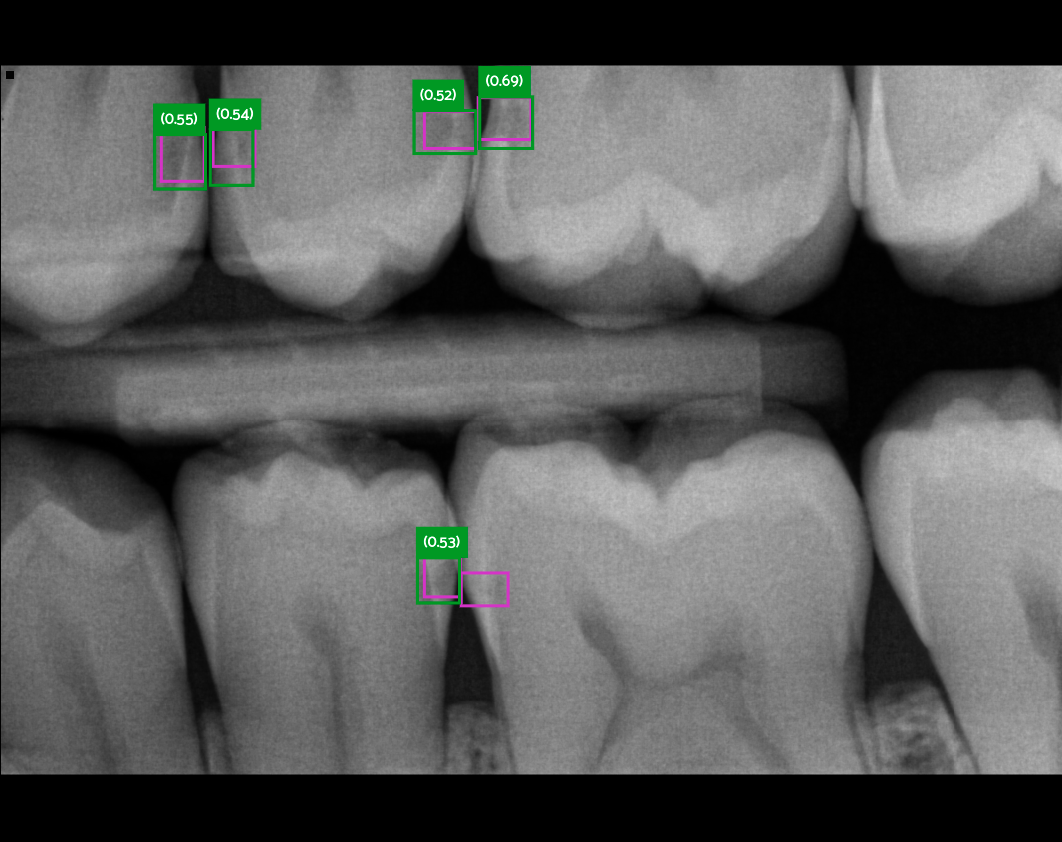
\includegraphics[width=0.9\linewidth]{images/no_rest2.png}
    \caption{X-ray image with ground truth boxes and model's predictions}
    \label{fig:pred_img2}
\end{figure}

\begin{figure}
    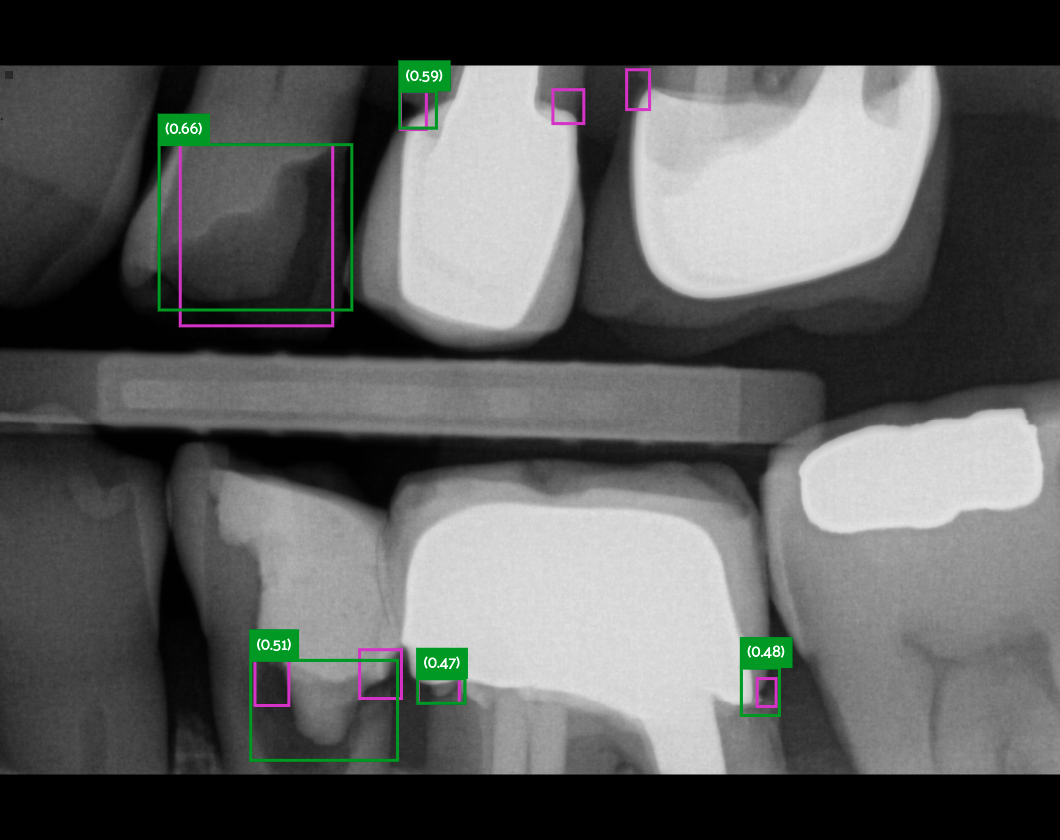
\includegraphics[width=0.9\linewidth]{images/rest1.png}
    \caption{X-ray image with ground truth boxes and model's predictions}
    \label{fig:pred_img3}
\end{figure}

\begin{figure}
    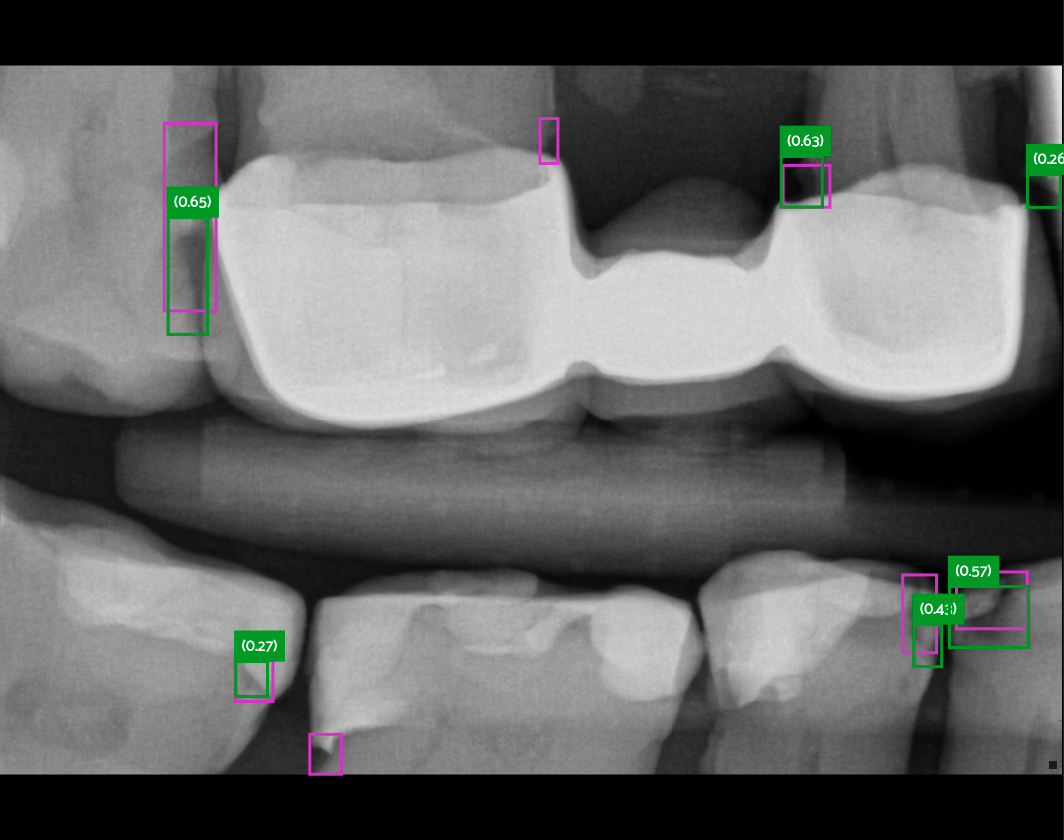
\includegraphics[width=0.9\linewidth]{images/rest2.png}
    \caption{X-ray image with ground truth boxes and model's predictions}
    \label{fig:pred_img4}
\end{figure}

\chapter{Augmented images}
\label{appendix:img_transformations}
\begin{figure}
    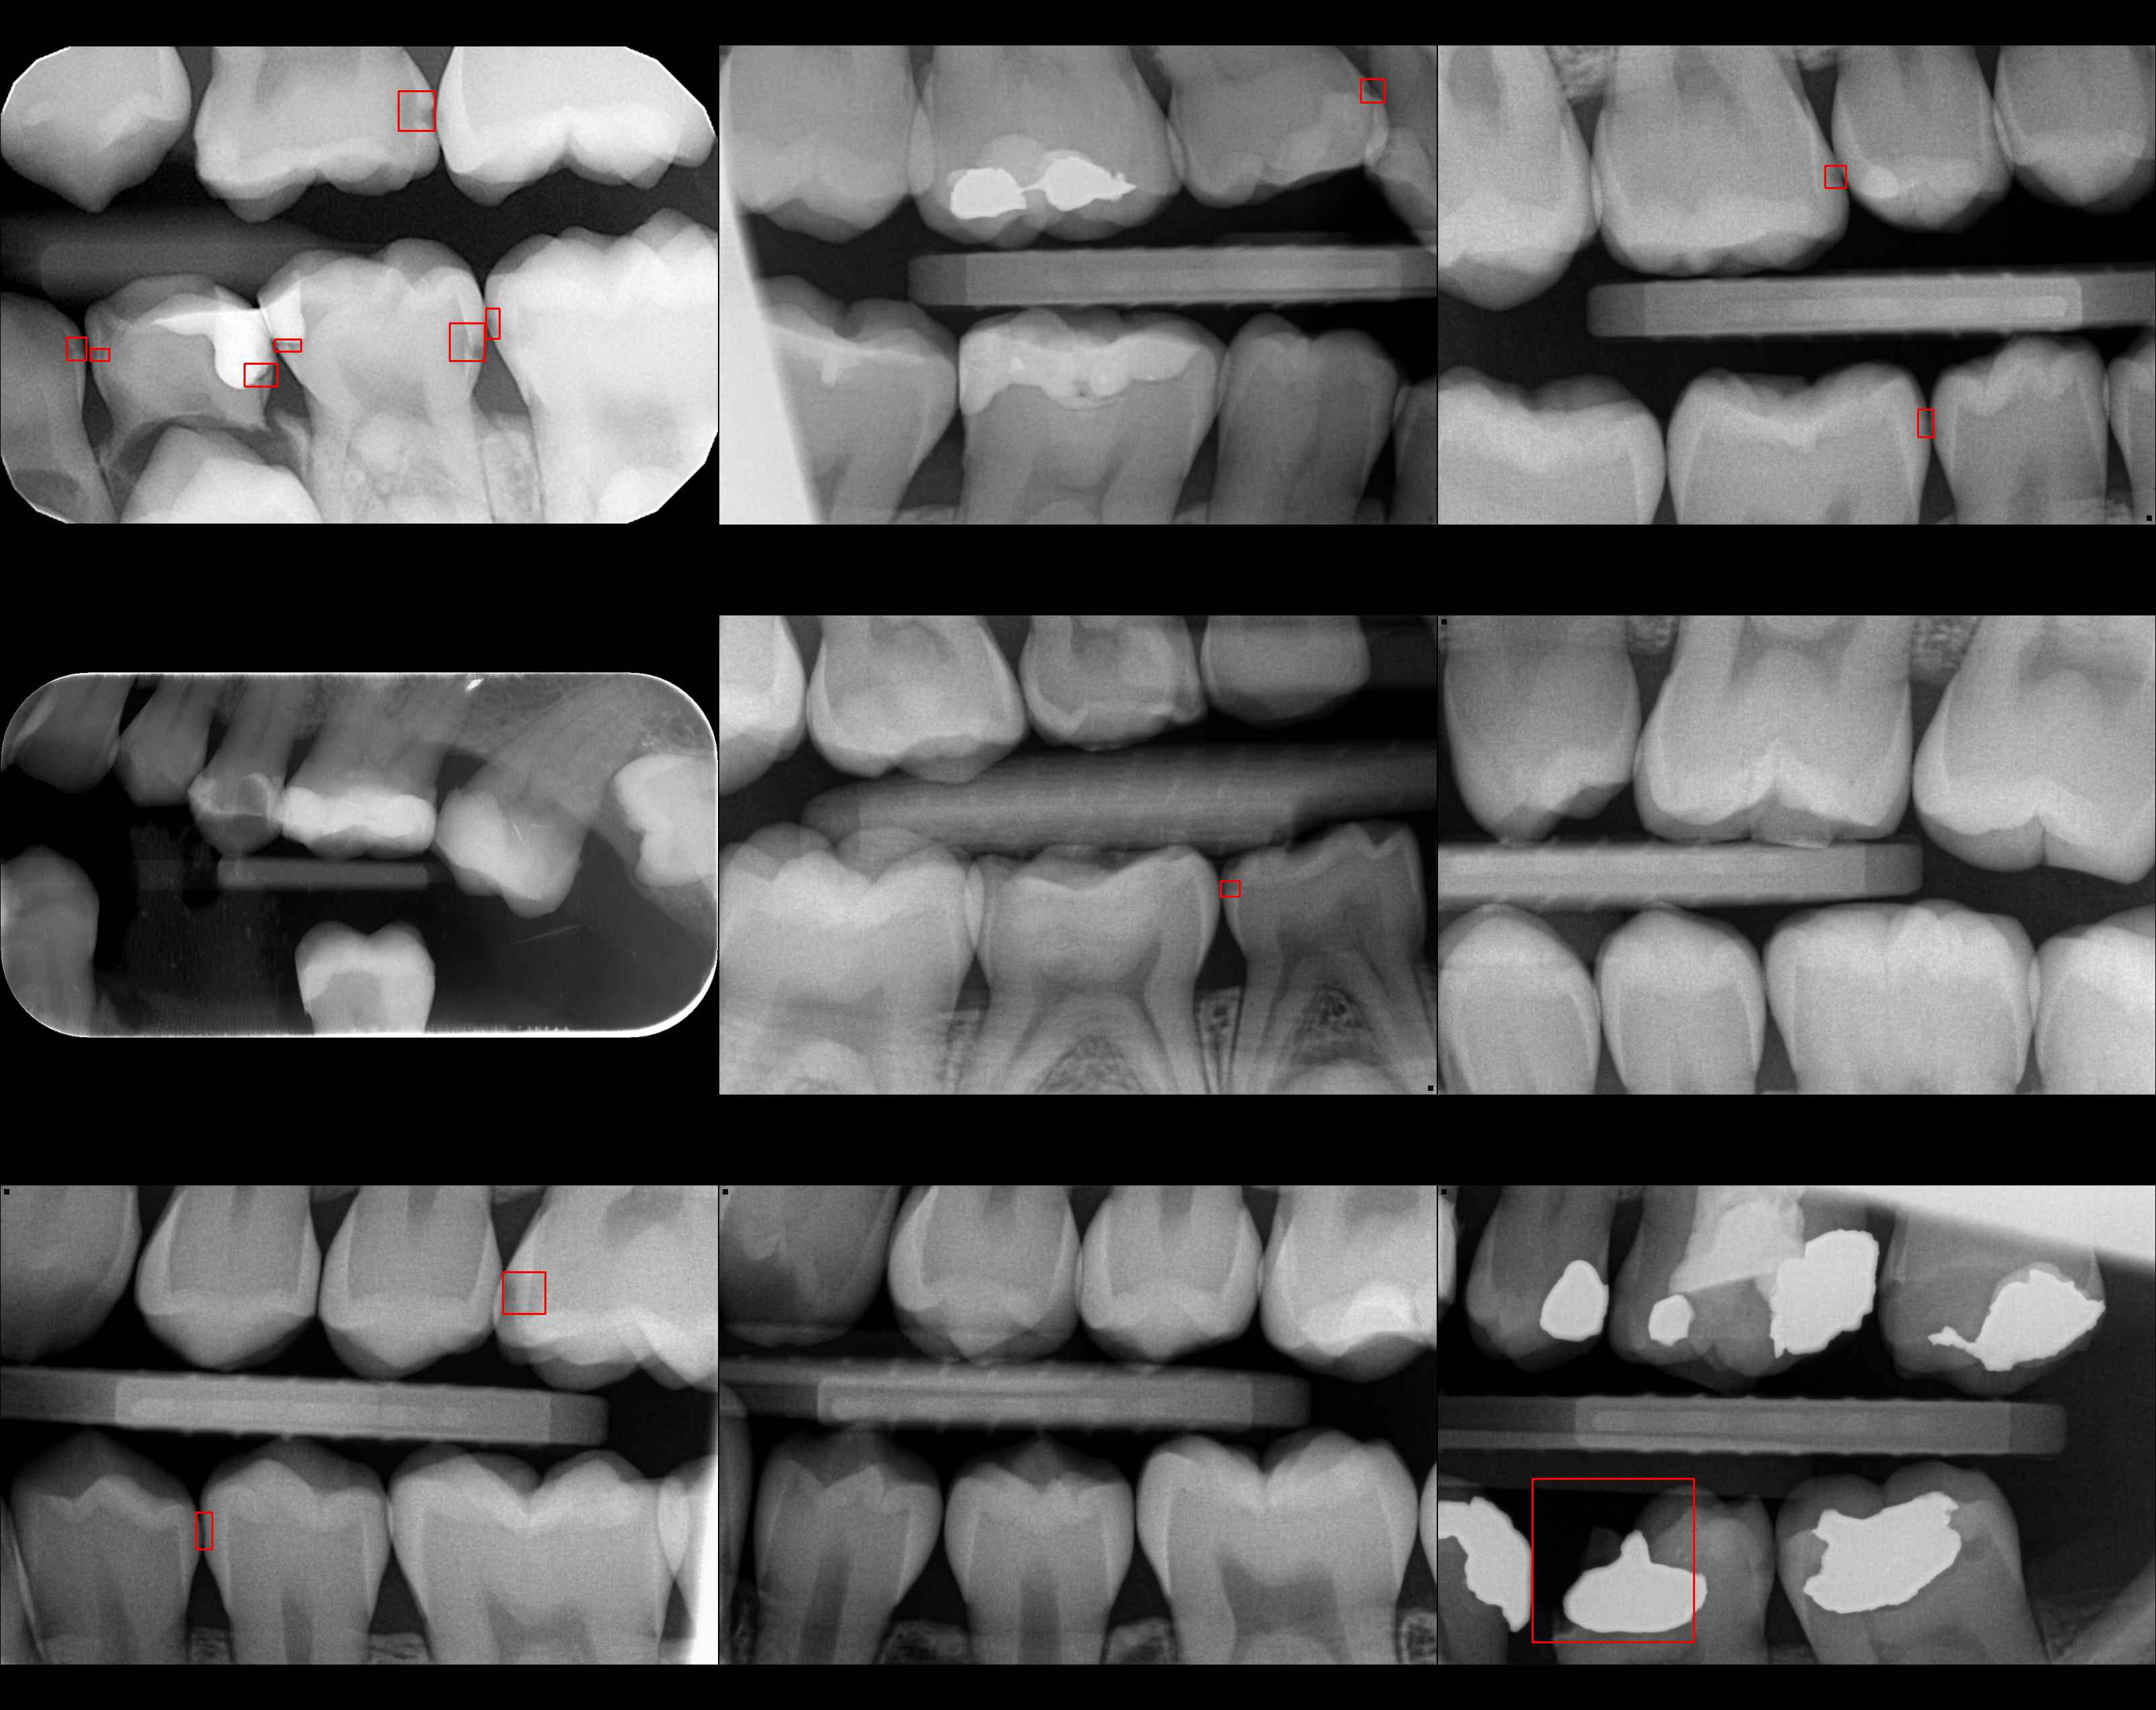
\includegraphics[width =0.9\linewidth]{images/no_trasnforms.jpg}
    \caption{No transformation applied}
\end{figure}
\begin{figure}
    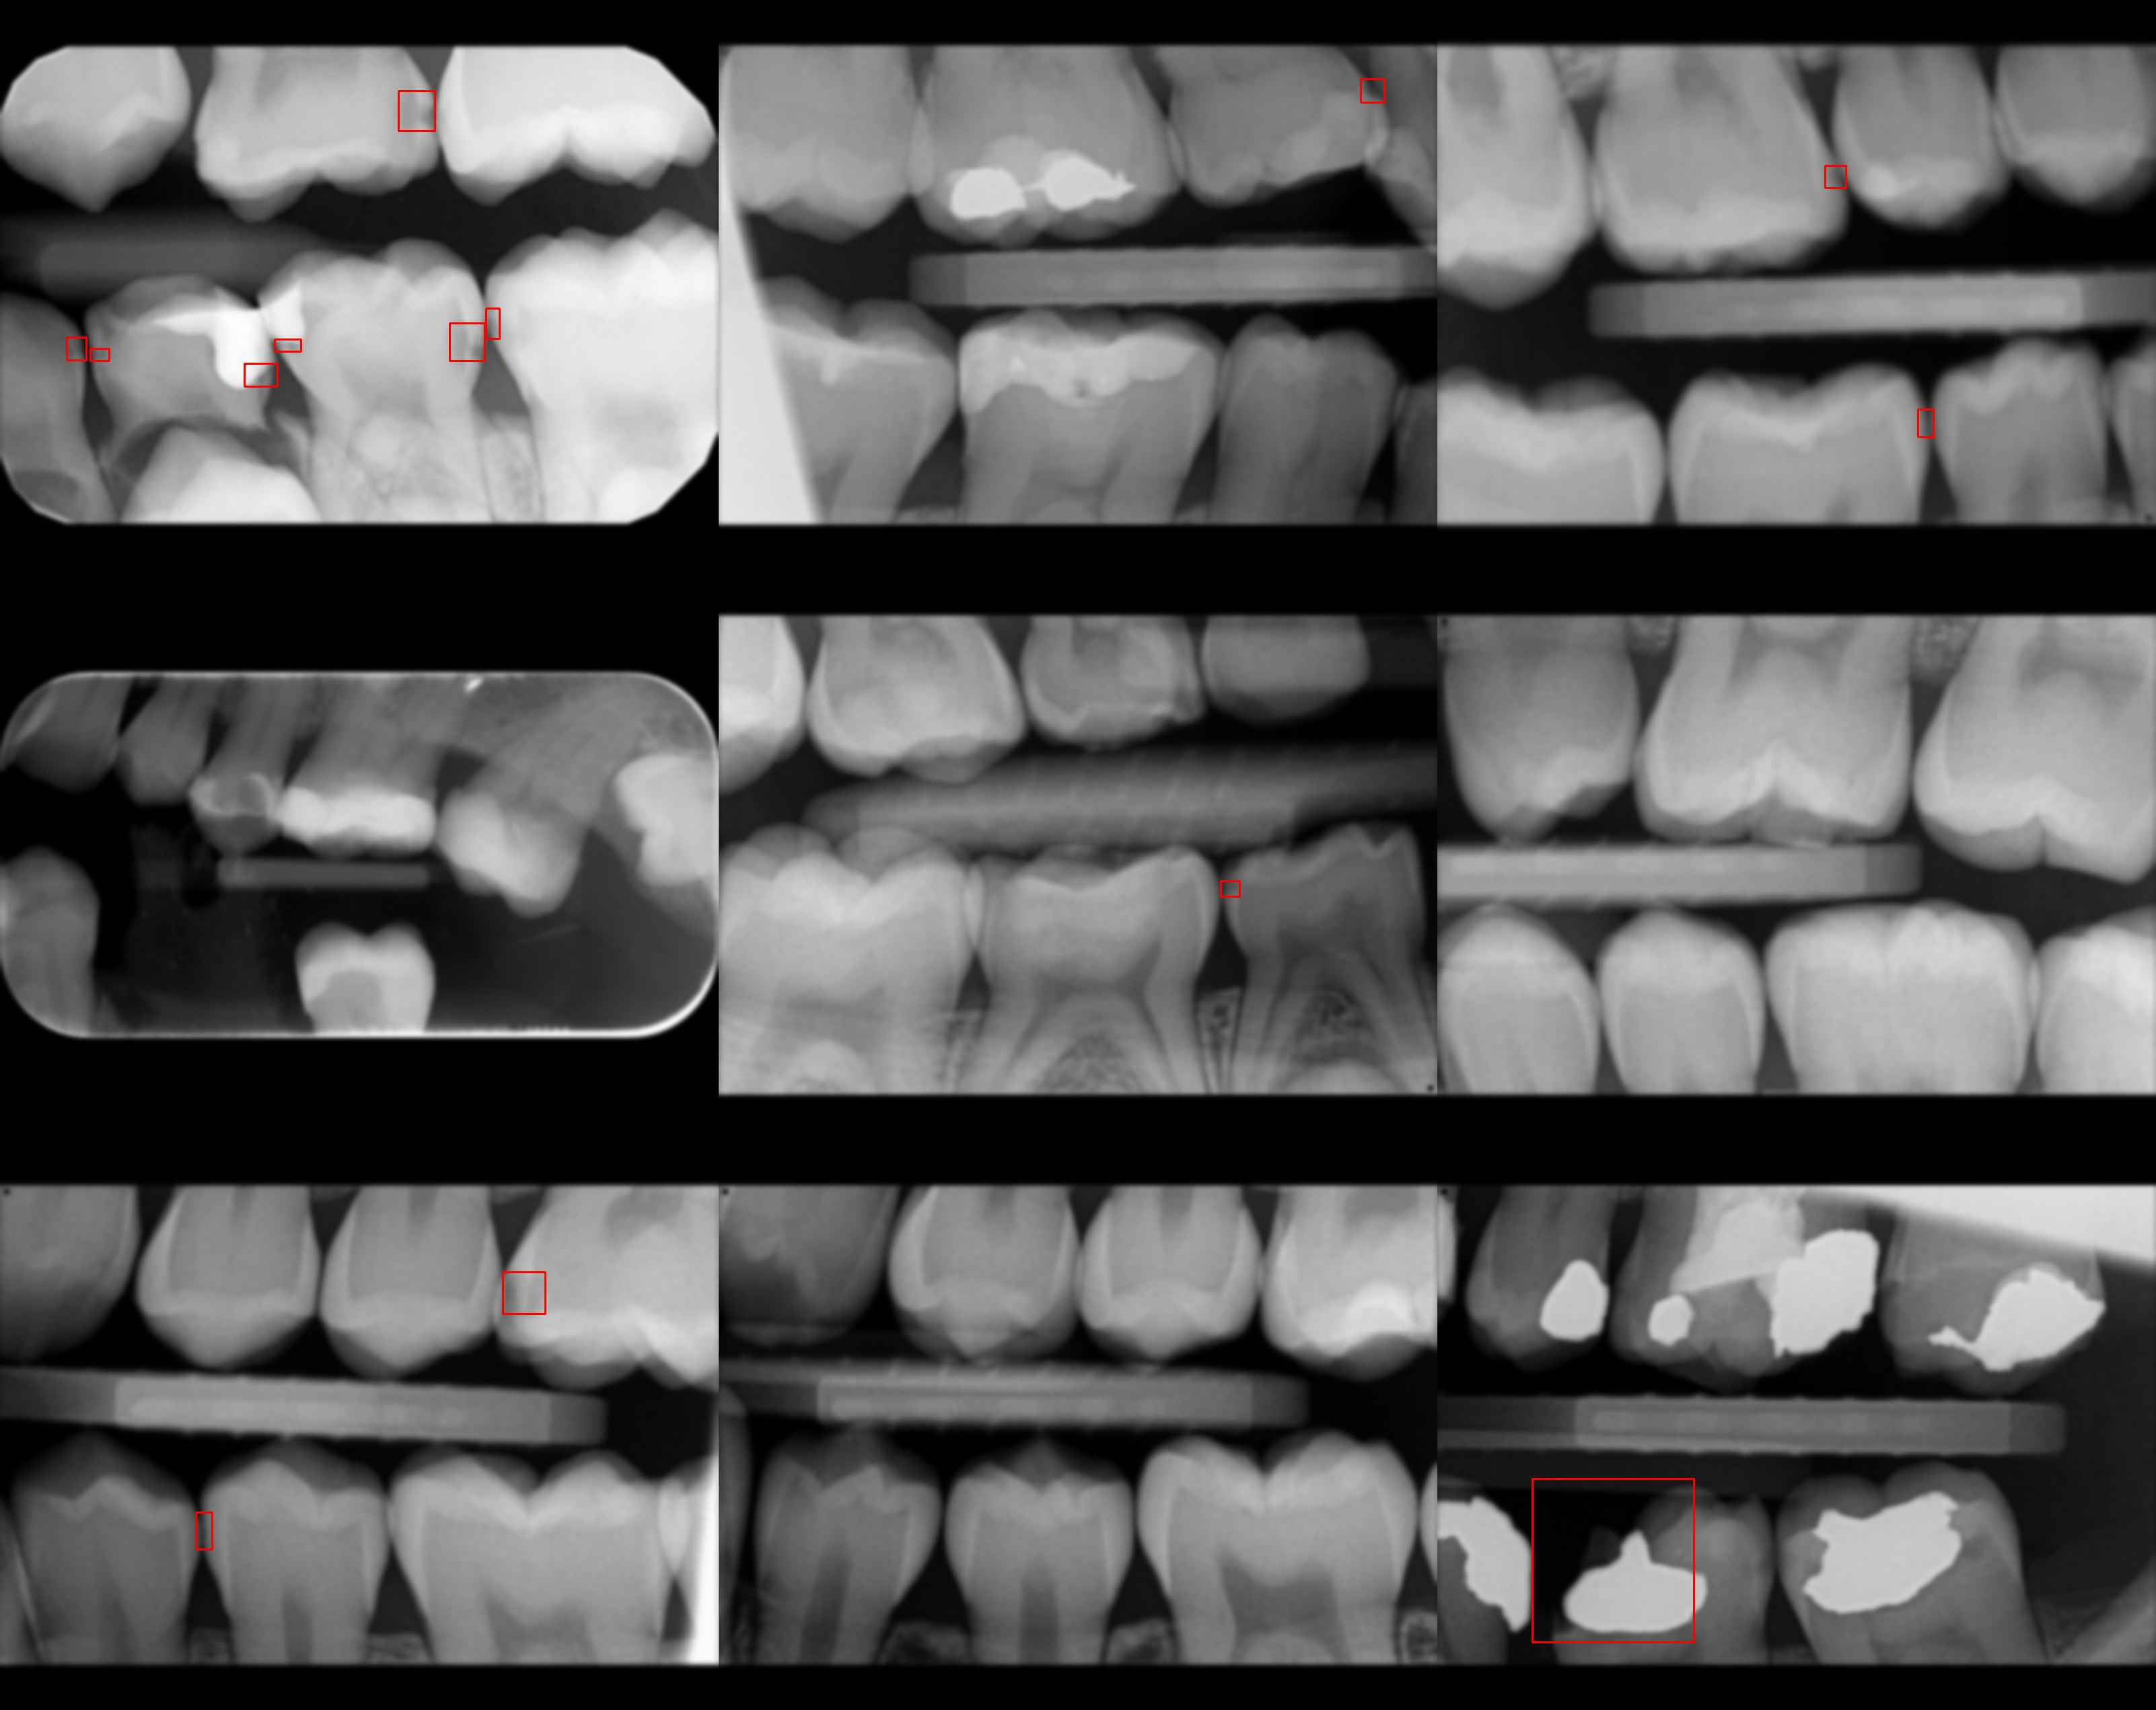
\includegraphics[width =0.9\linewidth]{images/gaussian_blur.jpg}
    \caption{Gaussian blur applied}
\end{figure}
\begin{figure}
    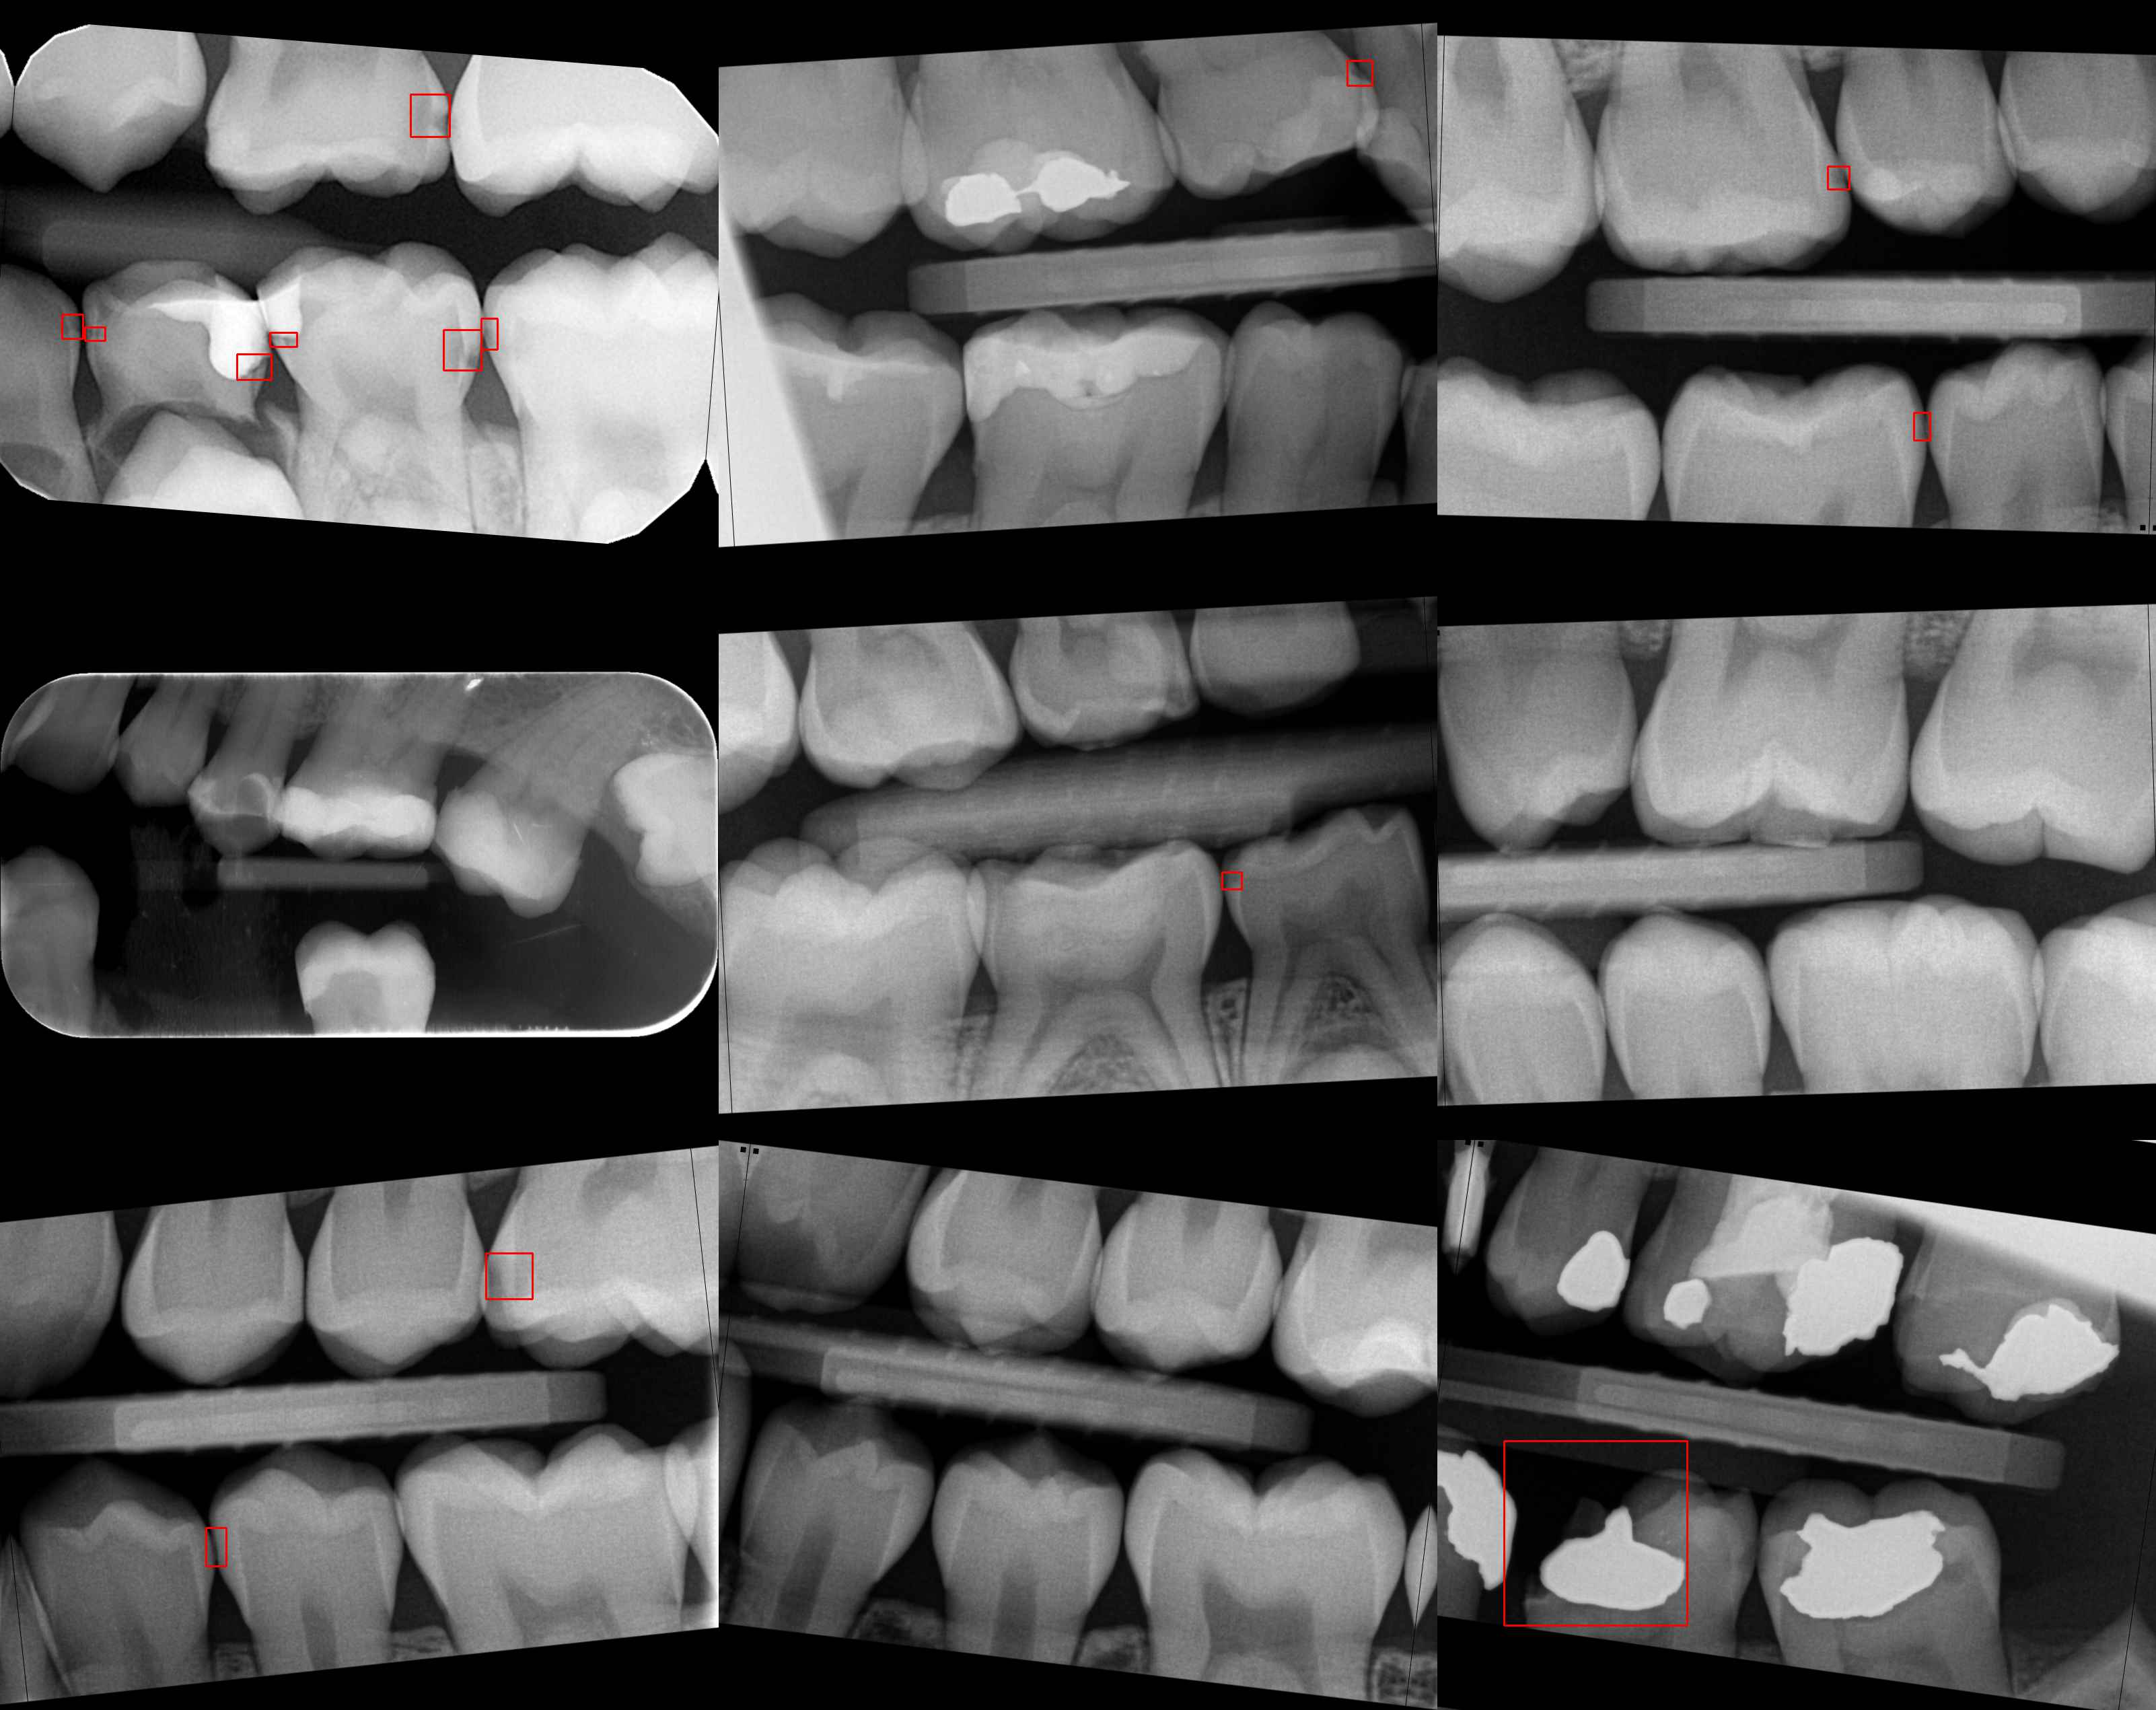
\includegraphics[width =0.9\linewidth]{images/roate_10.jpg}
    \caption{Rotation applied}
\end{figure}
\begin{figure}
    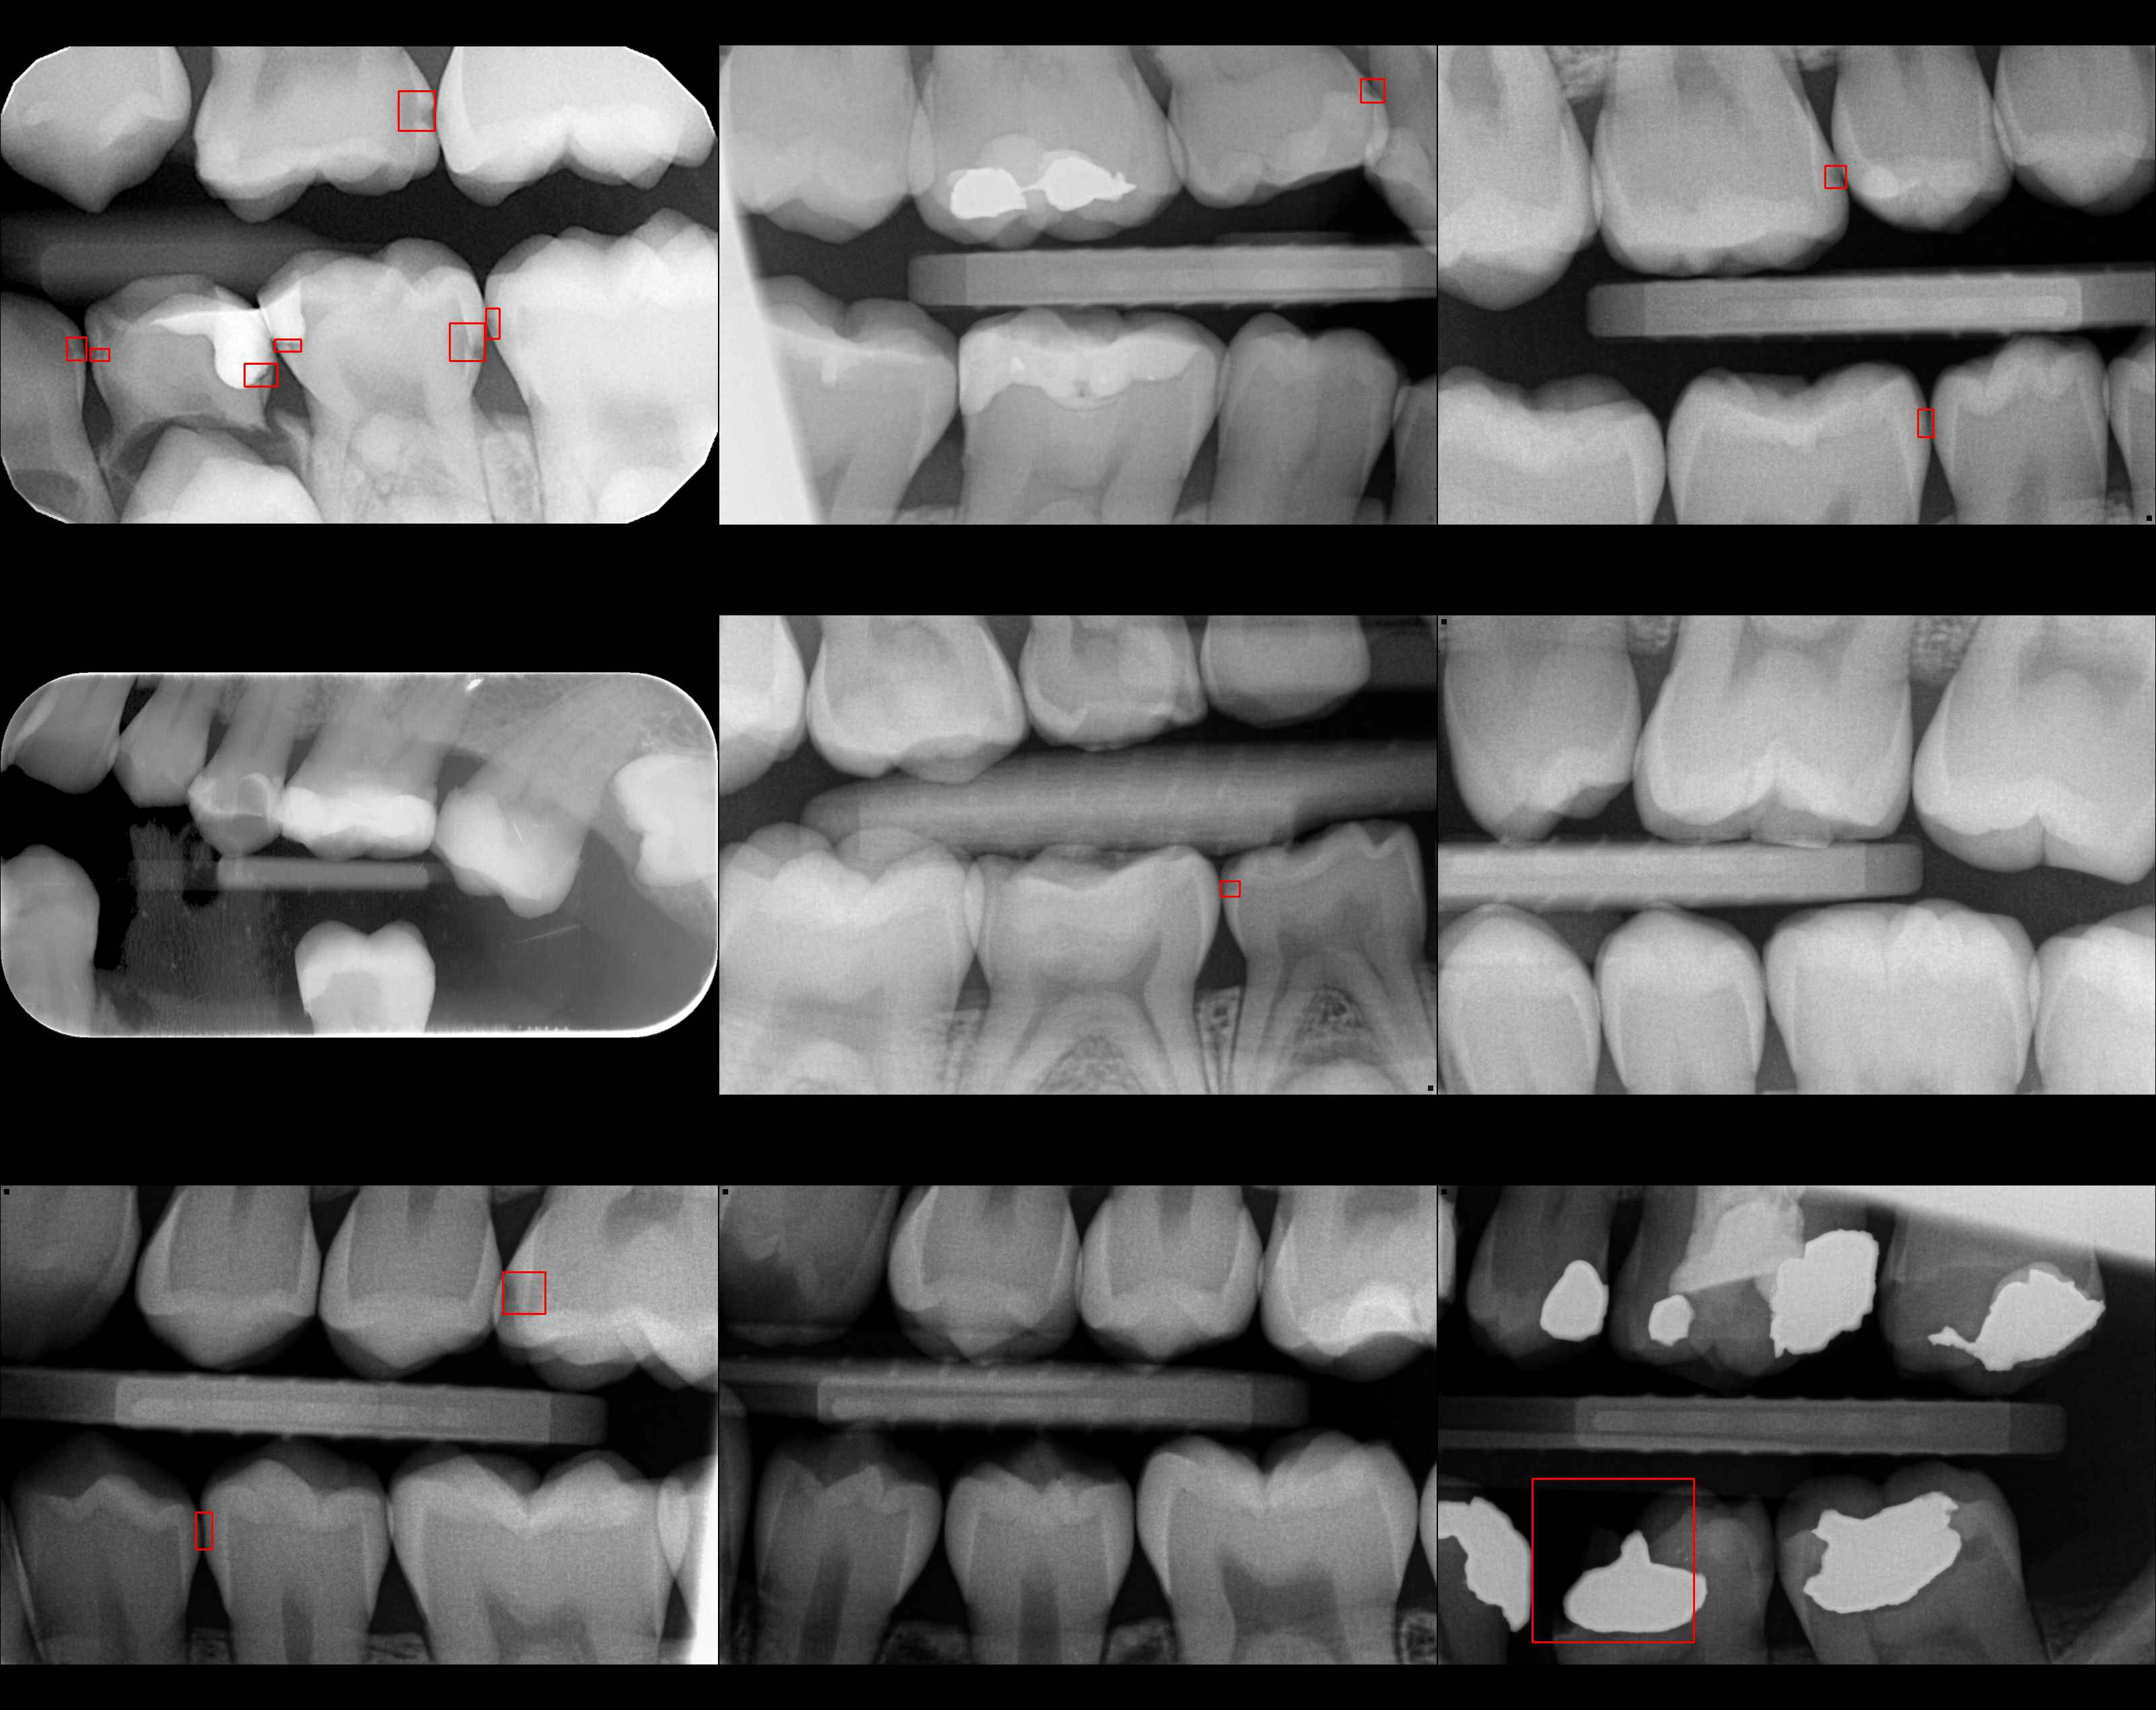
\includegraphics[width =0.9\linewidth]{images/random_gamma.jpg}
    \caption{Gamma correction applied}
\end{figure}
\begin{figure}
    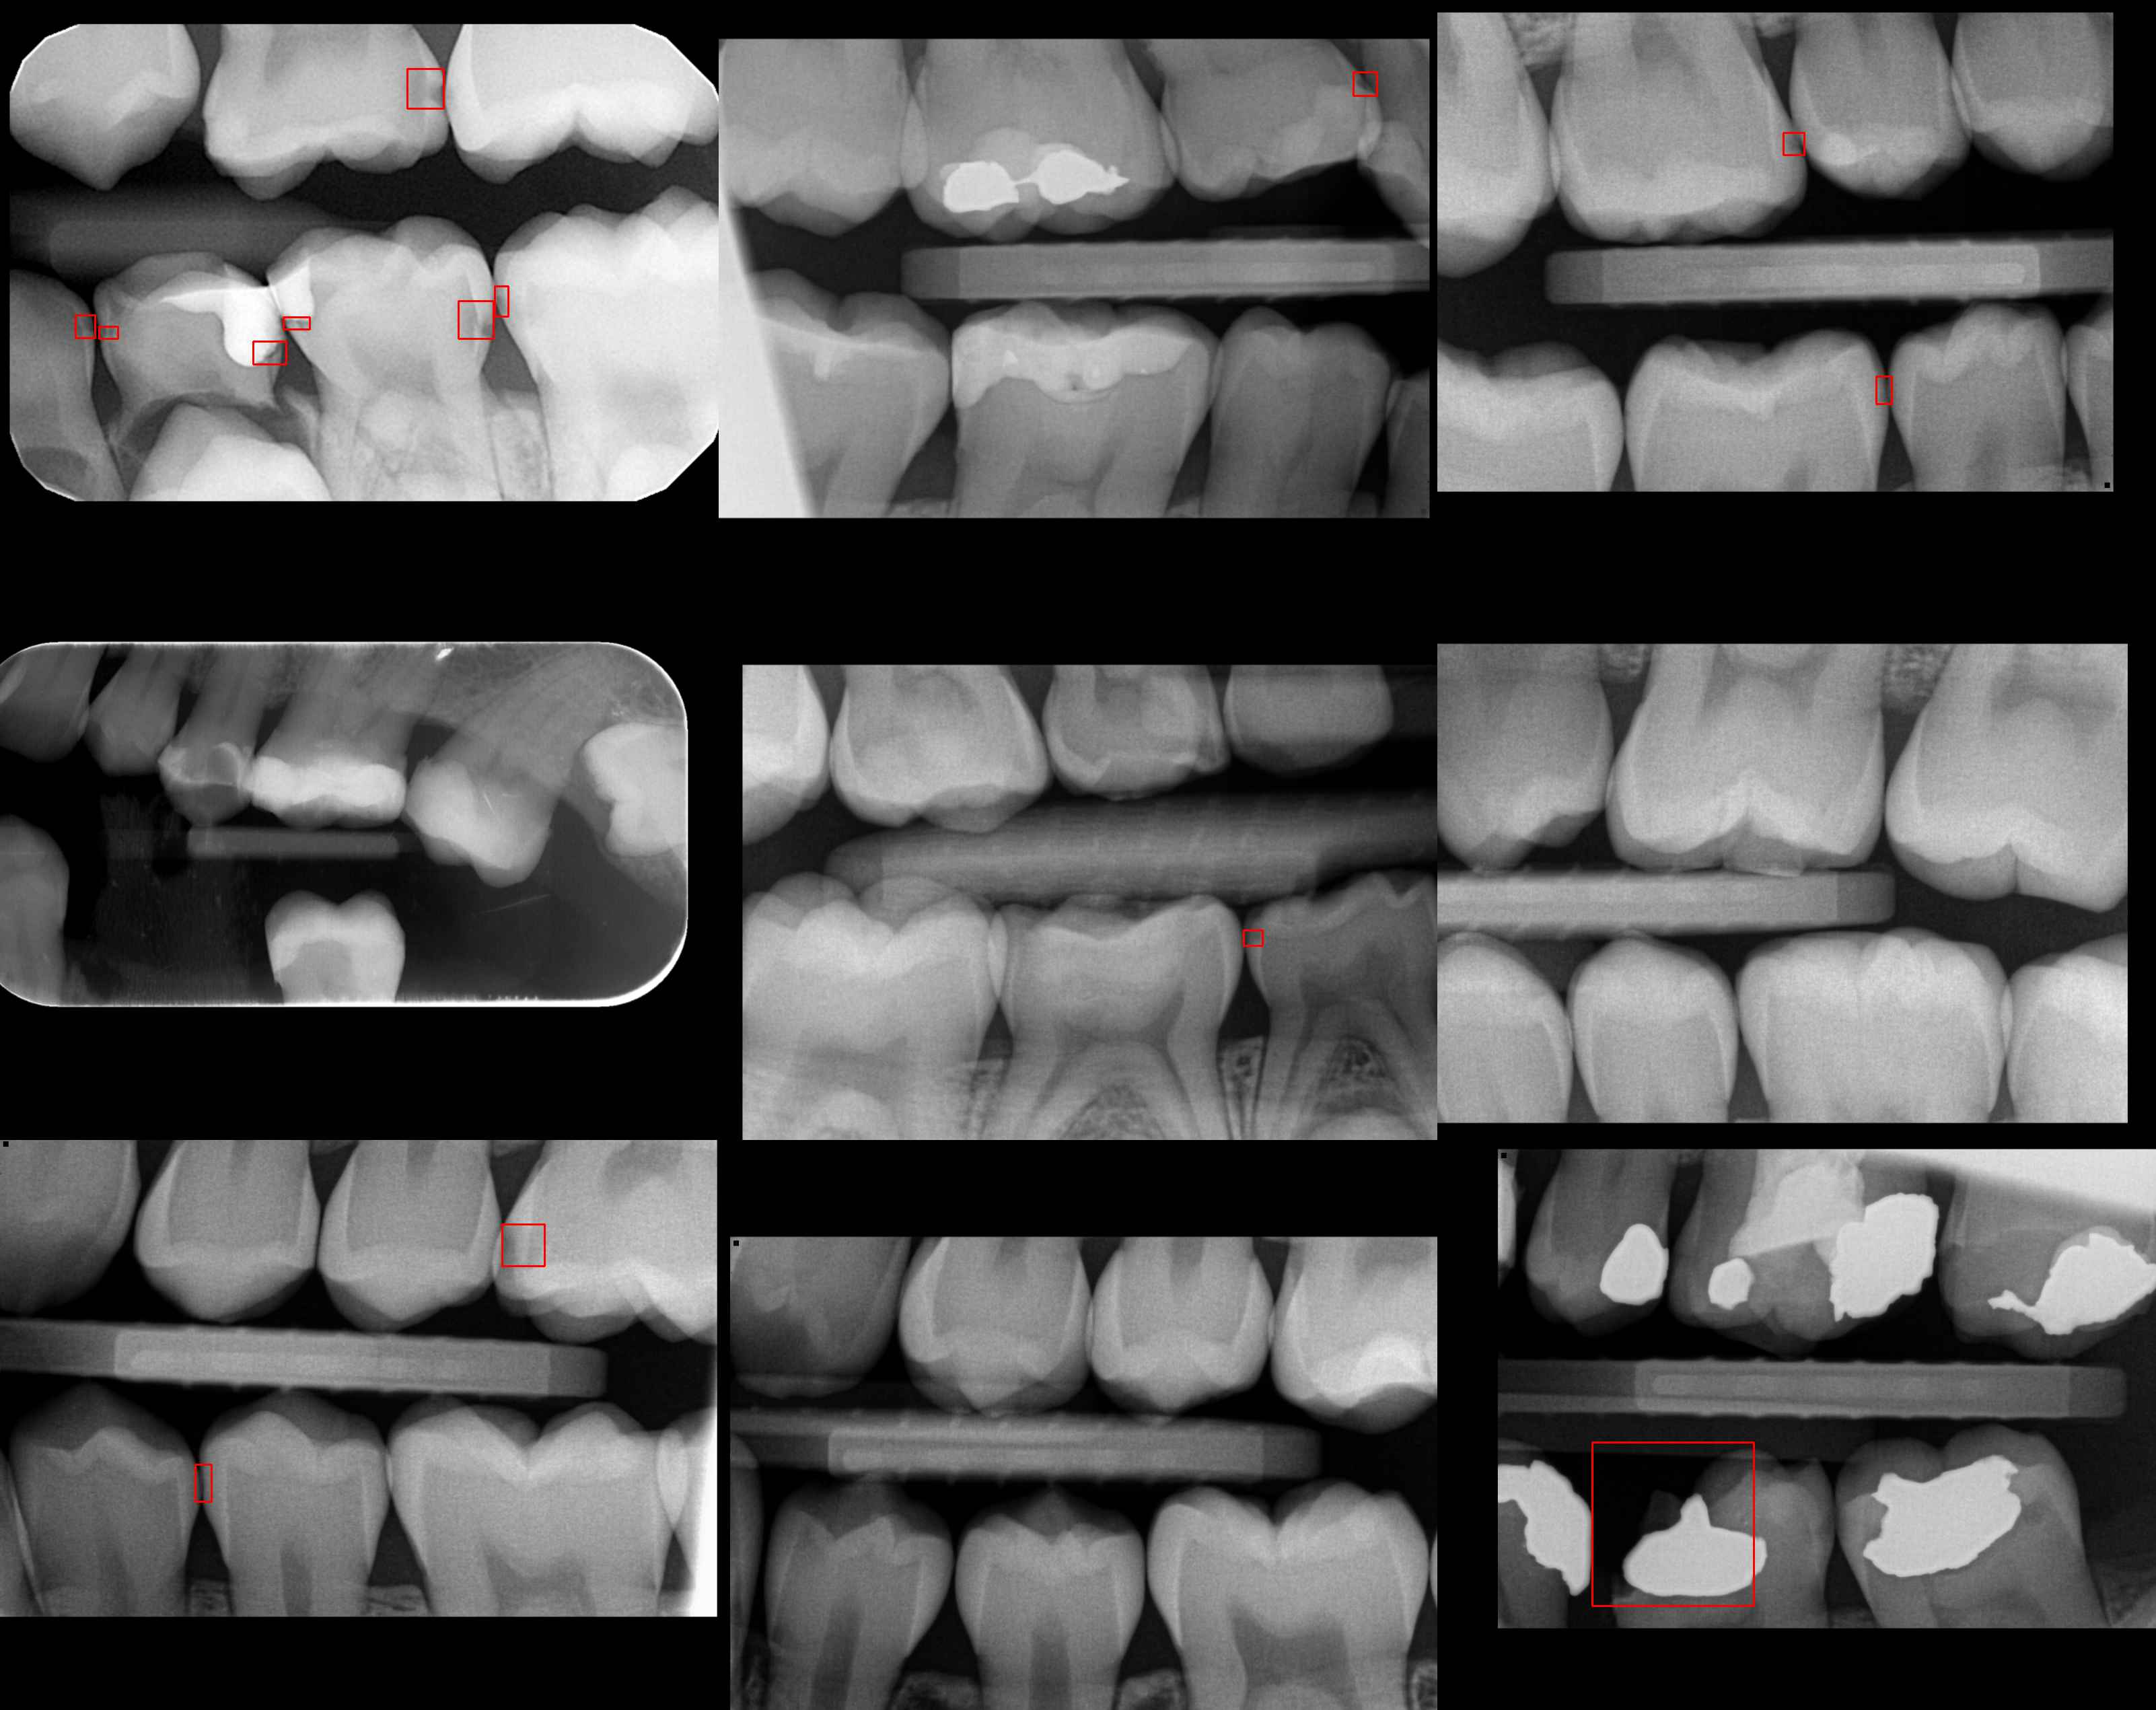
\includegraphics[width =0.9\linewidth]{images/translate.jpg}
    \caption{Translation applied}
\end{figure}
\begin{figure}
    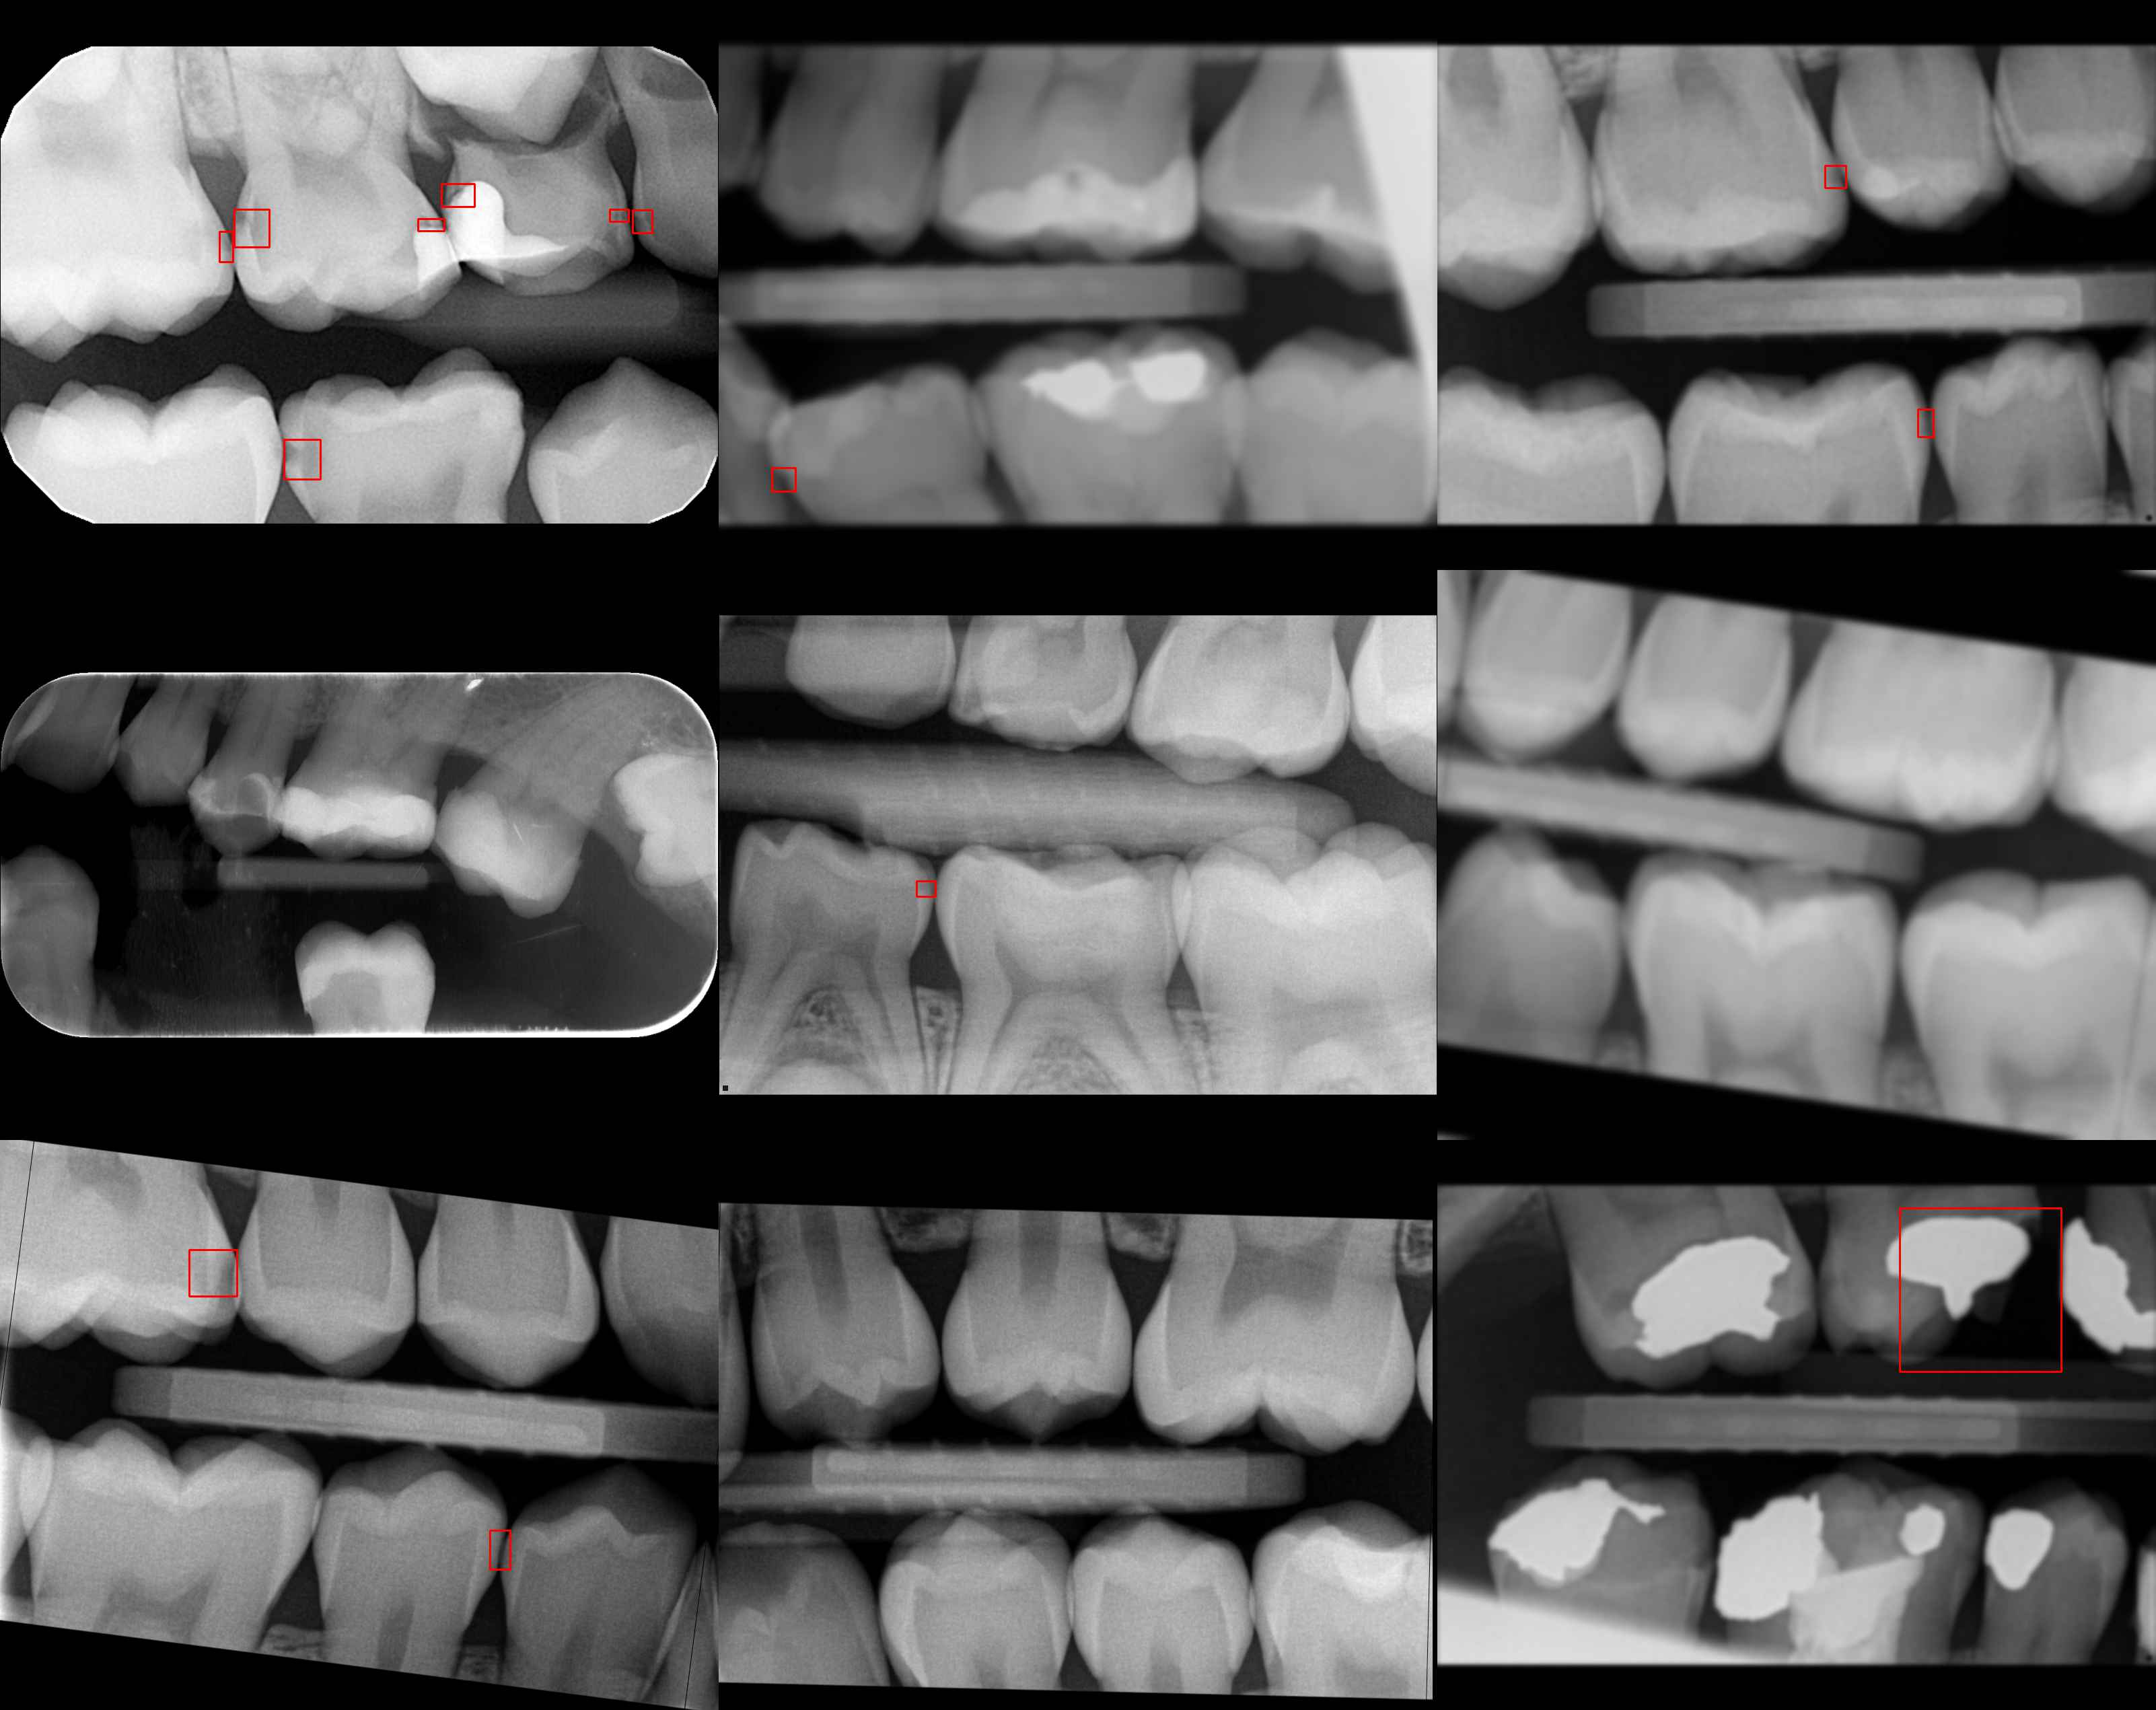
\includegraphics[width =0.9\linewidth]{images/all_transf.jpg}
    \caption{The whole augmentation pipeline applied}
\end{figure}